

%\documentclass[12pt]{article}
\documentclass[11pt]{scrartcl}
\title{EN2550_Assignment2}
\nonstopmode
%\usepackage[utf-8]{inputenc}
\usepackage{graphicx} % Required for including pictures
\usepackage[figurename=Figure]{caption}
\usepackage{float}    % For tables and other floats
\usepackage{verbatim} % For comments and other
\usepackage{amsmath}  % For math
\usepackage{amssymb}  % For more math
\usepackage{fullpage} % Set margins and place page numbers at bottom center
\usepackage{subcaption}
\usepackage{paralist} % paragraph spacing
\usepackage{listings} % For source code
\usepackage{subfig}   % For subfigures
%\usepackage{physics}  % for simplified dv, and 
\usepackage{enumitem} % useful for itemization
\usepackage{siunitx}  % standardization of si units
\usepackage{hyperref}
\usepackage{tikz,bm} % Useful for drawing plots
%\usepackage{tikz-3dplot}
\usepackage{circuitikz}

%%% Colours used in field vectors and propagation direction
\definecolor{mycolor}{rgb}{1,0.2,0.3}
\definecolor{brightgreen}{rgb}{0.4, 1.0, 0.0}
\definecolor{britishracinggreen}{rgb}{0.0, 0.26, 0.15}
\definecolor{cadmiumgreen}{rgb}{0.0, 0.42, 0.24}
\definecolor{ceruleanblue}{rgb}{0.16, 0.32, 0.75}
\definecolor{darkelectricblue}{rgb}{0.33, 0.41, 0.47}
\definecolor{darkpowderblue}{rgb}{0.0, 0.2, 0.6}
\definecolor{darktangerine}{rgb}{1.0, 0.66, 0.07}
\definecolor{emerald}{rgb}{0.31, 0.78, 0.47}
\definecolor{palatinatepurple}{rgb}{0.41, 0.16, 0.38}
\definecolor{pastelviolet}{rgb}{0.8, 0.6, 0.79}
\begin{document}

\begin{center}
	\hrule
	\vspace{.4cm}
	{\textbf { \large EN2550 --- Fundamentals of Image Processing and Machine Vision}}
\end{center}
{\textbf{Student Name:}\ Nuwan Bandara \hspace{\fill} \textbf{Submitted Date:} March 15, 2021   \\
{ \textbf{Student Number:}} \ 180066F \hspace{\fill} \textbf{Assignment Number:} 2 \\
	\hrule


\paragraph*{Problem 1} %\hfill \newline
Using the given code (item no. 1), experiment with various types of 2-D transformations. \newline
Image alignment is executed based on features and search sets of features match that agreed in terms of either local appearance or geometric configuration. Here, several 2D transformations are experimented using the given python implementation with different transformation matrices.

Entire code flow is executed and accessed on the Google Colaboratory platform (Colab) via (but, since Colab does not facilitate the OpenCV window sessions, the codes are experimented in local Jupyter environment and then, pasted in Colab), \\ 
\textbf{\url{https://colab.research.google.com/drive/1KxXmIZafbYoZzdW2Sy_iTmoo-EvR60NN?usp=sharing}}

\begin{equation}
H_{Euclidean} = 
\begin{bmatrix}
\cos{\theta} & -\sin{\theta} & t_x\\
\sin{\theta} & \cos{\theta} & t_y\\
0 & 0 & 1
\end{bmatrix}, H_{Similarity}=
\begin{bmatrix}
s\cos{\theta} & -s\sin{\theta} & t_x\\
s\sin{\theta} & s\cos{\theta} & t_y\\
0 & 0 & 1
\end{bmatrix}
\end{equation}

\begin{equation}
    H_{Simplified Affine}=
\begin{bmatrix}
1 & \tan{\theta} & t_x\\
\tan{\theta} & 1 & t_y\\
0 & 0 & 1
\end{bmatrix}
\end{equation}

\begin{figure}[H]
\centering
\begin{subfigure}{.5\textwidth}
  \centering
  \includegraphics[width=0.9\linewidth]{Euclidean.PNG}
  \caption{Euclidean transformation matrix}
  \label{fig:sub1}
\end{subfigure}%
\begin{subfigure}{0.5\textwidth}
  \centering
  \includegraphics[width=0.9\linewidth]{Similarity.PNG}
  \caption{Similarity transformation matrix}
  \label{fig:sub2}
\end{subfigure}
\caption{Python implementations of 2D transformation matrices}
\label{fig:test}
\end{figure}

\begin{figure}[h!]
\centering
\begin{subfigure}{.5\textwidth}
  \centering
  \includegraphics[width=.4\linewidth]{Euclidean1.PNG}
  \caption{After Euclidean transformation}
  \label{fig:sub1}
\end{subfigure}%
\begin{subfigure}{0.5\textwidth}
  \centering
  \includegraphics[width=.4\linewidth]{Similarity1.PNG}
  \caption{After Similarity transformation}
  \label{fig:sub2}
\end{subfigure}
\caption{Results after 2D transformations}
\label{fig:test}
\end{figure}

\begin{figure}[h!]
\centering
\begin{subfigure}{0.5\textwidth}
  \centering
  \includegraphics[width=.5\linewidth]{ShearX.PNG}
  \caption{After Shear transformation in x-direction}
  \label{fig:sub2}
\end{subfigure}
\begin{subfigure}{0.4\textwidth}
  \centering
  \includegraphics[width=.3\linewidth]{ShearY.PNG}
  \caption{After Shear transformation in y-direction}
  \label{fig:sub2}
\end{subfigure}
\begin{subfigure}{0.4\textwidth}
  \centering
  \includegraphics[width=.5\linewidth]{ShearXY.PNG}
  \caption{After Simplified Affine transformation}
  \label{fig:sub2}
\end{subfigure}
\caption{Results after 2D transformations (Problem 1)}
\label{fig:test}
\end{figure}


\paragraph*{Problem 2}
Transform Graffiti (https://www.robots.ox.ac.uk/~vgg/data/affine/) img1.ppm onto img5.ppm
using code in item no. 2.

In order to apply perspective transformation, a 3x3 transformation matrix is needed. This transformation matrix could be calculated using OpenCV inbuilt \textit{getPerspectiveTransform} by referring four points on the input image and corresponding points on the output image. Here, the transformation matrix is given in the \textit{H1to5p} file and the requirement is to apply this matrix using \textit{warpPerspective} function which gets input image, output image (im4), transformation matrix (H), size of the output image ((1000x1000)), combination of interpolation methods, pixel extrapolation method and boarder value as input parameters. Afterwards, the warped image is stitched with the input im1 image as per given in the code. Here, the variants necessarily includes coordinates of quadrangle vertices in the source image and coordinates of the corresponding quadrangle vertices in the destination image.
\begin{figure}[H]
\centering
\begin{subfigure}{0.4\textwidth}
  \centering
  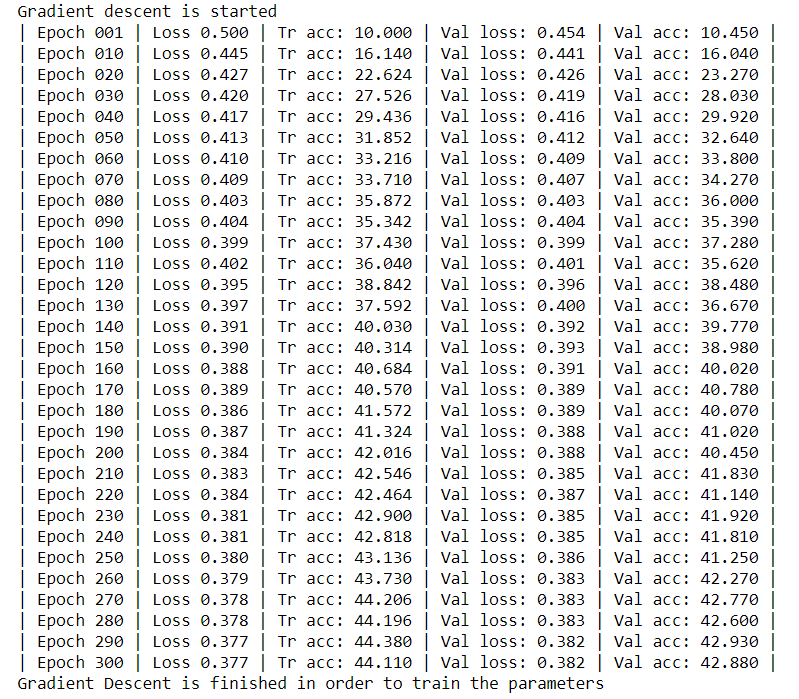
\includegraphics[width=.5\linewidth]{2_1.PNG}
  \caption{Input Image - img1.ppm}
  \label{fig:sub2}
\end{subfigure}
\begin{subfigure}{0.4\textwidth}
  \centering
  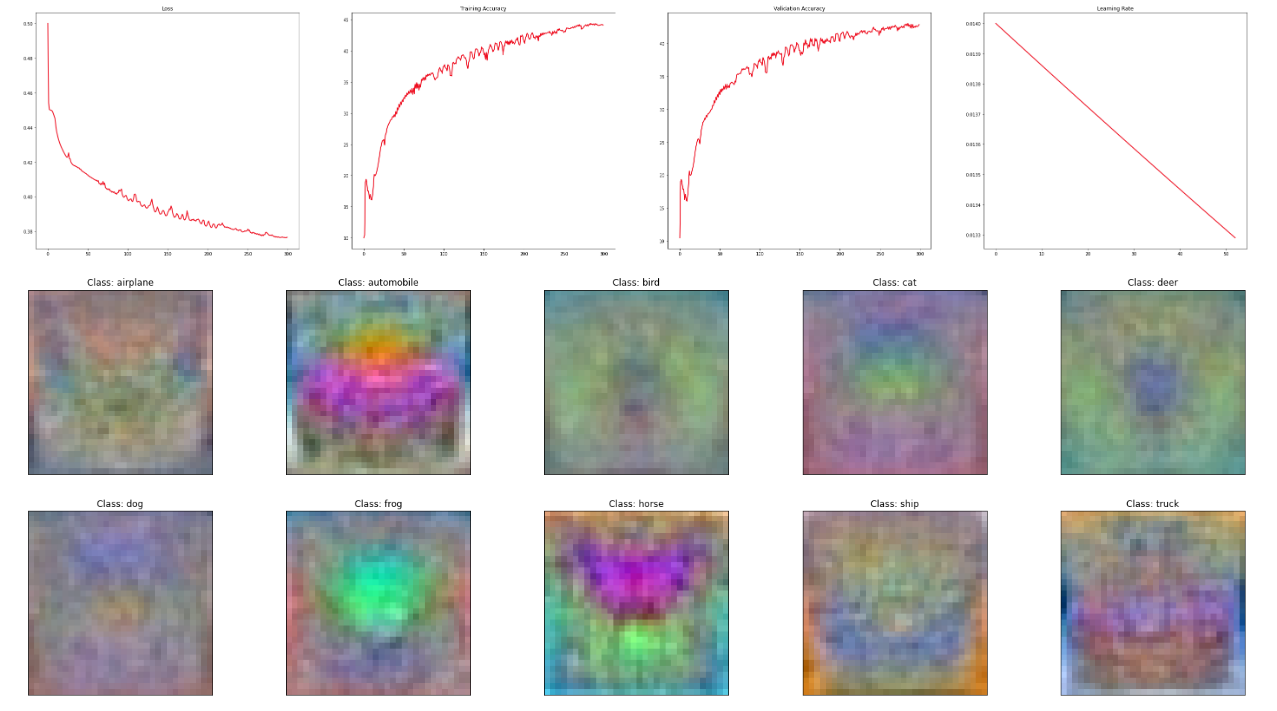
\includegraphics[width=.5\linewidth]{2_2.PNG}
  \caption{Image 5 - img5.ppm}
  \label{fig:sub2}
\end{subfigure}
\begin{subfigure}{0.4\textwidth}
  \centering
  \includegraphics[width=.5\linewidth]{2_3.PNG}
  \caption{Image 5 warped image}
  \label{fig:sub2}
\end{subfigure}
\caption{Before and after transformation}
\label{fig:test}
\end{figure}


\paragraph*{Problem 3}
Item no. 3 is for mouse clicking and selecting matching points in the two images to be stitched. Compute the homography using the relevant OpenCV function and carry out stitching.

In the the projective transformation, the planar homography relates the transformation between two planes (up to a scale factor) such that,
\begin{equation}
H 
\begin{bmatrix}
x\\
y\\
1
\end{bmatrix} =
\begin{bmatrix}
h_{11} & h_{12} & h_{13}\\
h_{21} & h_{22} & h_{23}\\
h_{31} & h_{32} & h_{33}
\end{bmatrix}
\begin{bmatrix}
x\\
y\\
1
\end{bmatrix}
\end{equation}
This homography matrix is contained with eight degrees of freedom (thus, requires four corresponding points) and in general, normalized with,
\begin{equation}
    h_{33}=1 \hspace{2mm} or \hspace{2mm} h^2_{11}+h^2_{12}+h^2_{13}+h^2_{21}+h^2_{22}+h^2_{23}+h^2_{31}+h^2_{32}+h^2_{33}=1
\end{equation}
The crucial invariant in homography is the cross ratio of four co-linear points (ratio of ratios of lengths) and if $h_{33}=0$ and having n-points, such that,
\begin{equation}
    \begin{bmatrix}
    \textbf{$0^T$} & \textbf{$x^T_1$} & ... & \textbf{$-y^1_1x^T_1$}\\
    \textbf{$x^T_1$} & \textbf{$0^T$} & ... & \textbf{$-x^1_1x^T_1$}\\
        ...
    \\
    ...\\
    \textbf{$0^T$} & \textbf{$x^T_n$} & ... & \textbf{$-y^1_nx^T_n$}\\
    \textbf{$x^T_n$} & \textbf{$0^T$} & ... & \textbf{$-x^1_nx^T_n$}
    \end{bmatrix}_{2n*9}\begin{bmatrix}
    h_1\\h_2\\h_3
    \end{bmatrix}_{9*1}=
    \begin{bmatrix}
    0\\0\\...\\...\\0
    \end{bmatrix}_{2n*1}
\end{equation}
In the form of $Ah=0$. Hence, the solution would be the unit eigen vector of $A_TA$ corresponding to the smallest eigen value.

The inbuilt OpenCV function \textit{findHomography} which gets \textit{object Points Planar} and \textit{image points} as input parameters could easily be used to estimate or compute the homography as implemented below.

\begin{figure}[H]
    \centering
    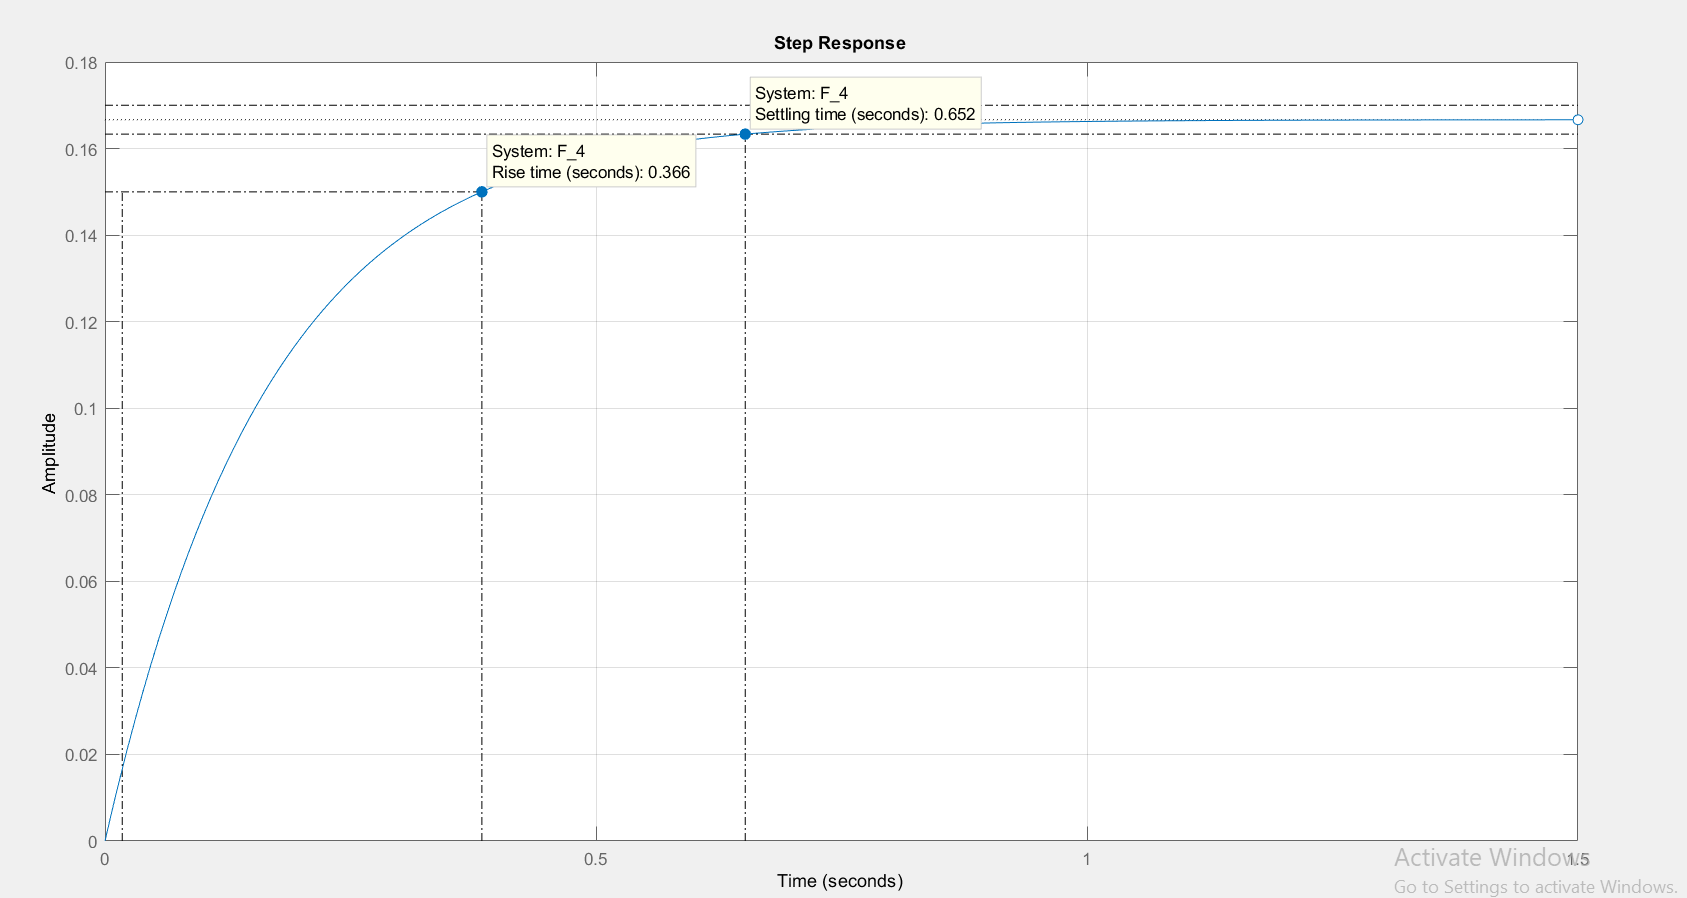
\includegraphics[width=0.6\textwidth]{3_1.PNG}
    \caption{OpenCV inbuilt function implementation to compute homography}
    \label{fig: PaleBlueDot}    
\end{figure}

Afterwards, as in problem (3), the \textit{warpPerspective} is utilized in order to apply the obtained transformation into stitching as per required.

\begin{figure}[H]
\centering
\begin{subfigure}{0.4\textwidth}
  \centering
  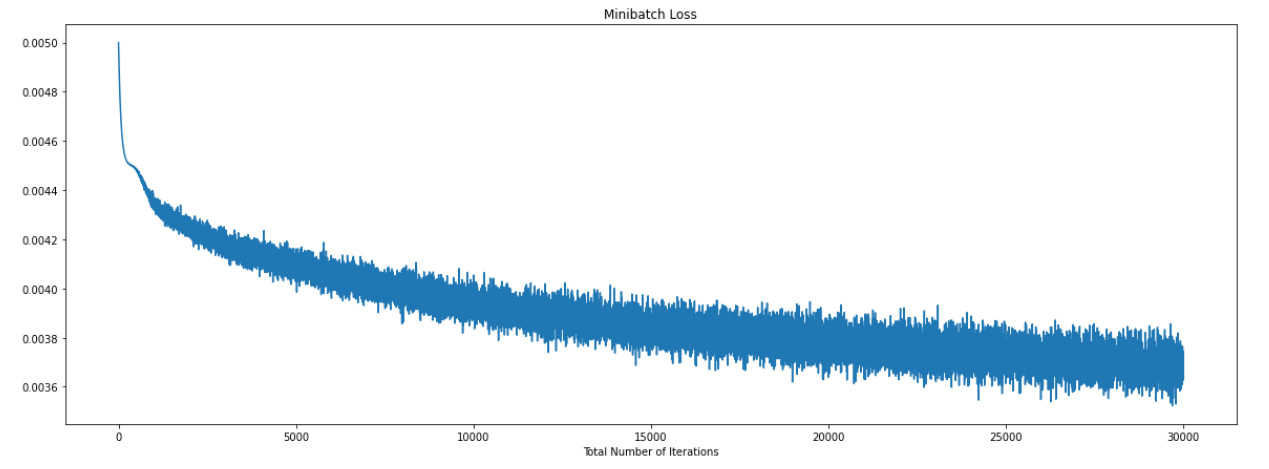
\includegraphics[width=.5\linewidth]{3_2.PNG}
  \caption{Input Image - img1.ppm}
  \label{fig:sub2}
\end{subfigure}
\begin{subfigure}{0.4\textwidth}
  \centering
  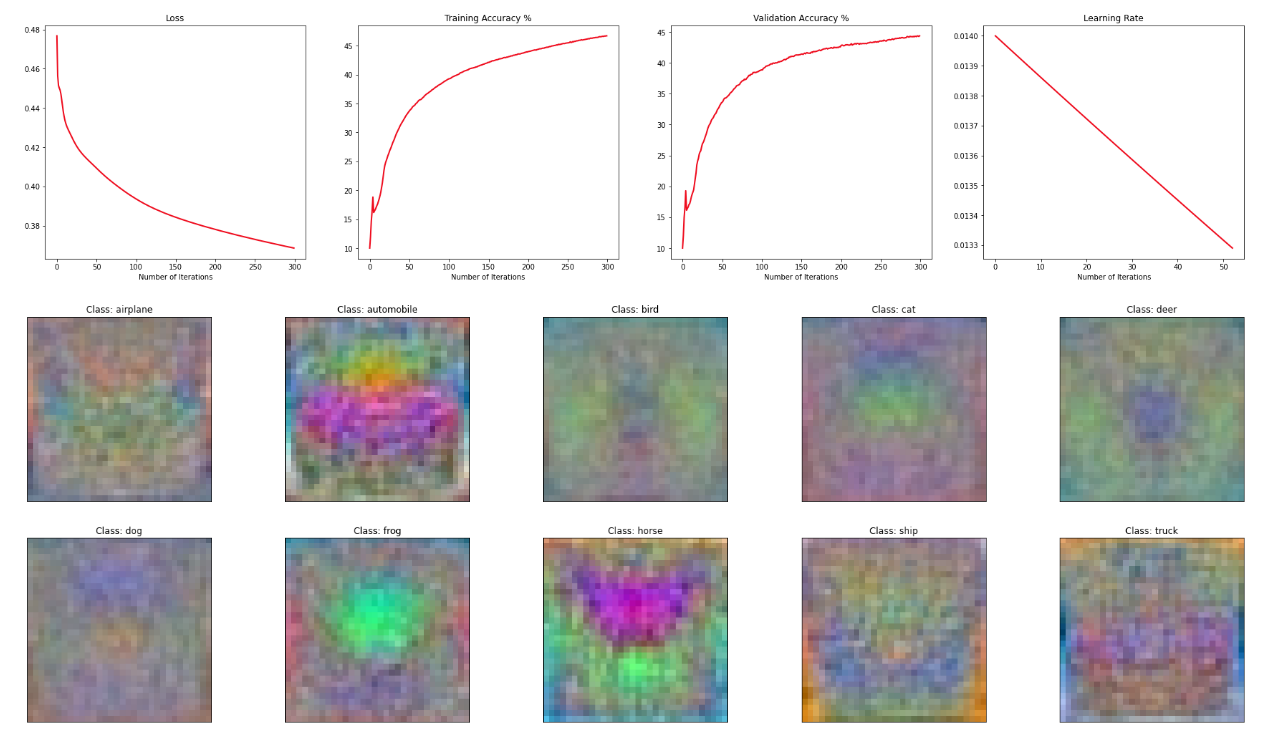
\includegraphics[width=.5\linewidth]{3_3.PNG}
  \caption{Image 5 - img5.ppm}
  \label{fig:sub2}
\end{subfigure}
\begin{subfigure}{0.4\textwidth}
  \centering
  \includegraphics[width=.5\linewidth]{3_4.PNG}
  \caption{Image 1 warped image}
  \label{fig:sub2}
\end{subfigure}
\caption{Before and after stitching}
\label{fig:test}
\end{figure}

The obtained warped image suggests that the perspective transformation by computing homography (using the OpenCV inbuilt function) is working perfectly in this problem since it seems almost similar with the original image 5 with no significant distortion.

\paragraph*{Problem 4}
Item no. 4 is similar to item no. 3. Here, compute the homography using your own code and stitch the two images.

In order to compute the homography using a custom function, the equation (5) is utilized as the reference. 

In this code, first, the required matrices are defined as per zero arrays with the corresponding shapes as referenced. Afterwards, the specific values for the each element in matrix A has been assigned using the input parameters to the custom function  which are the simply the corresponding mouse-clicked points.

In the assigning process of values to the corresponding elements in matrix A, an estimation has been induced to the even and odd rows in certain columns as assigning values of 0 and 1 as assumed. Afterwards, the singular value decomposition is utilized via \textit{numpy linalg.svd} in order to obtain the necessary values for the transformation matrix H.

Afterwards, the obtained H matrix is reshaped into the shape of (3x3) since the function \textit{warpPerspective} needs the transformation matrix to be in that shape. The rest of the code is similar with the previously applied implementation in problem (3).

\begin{figure}[H]
\centering
\begin{subfigure}{0.4\textwidth}
  \centering
  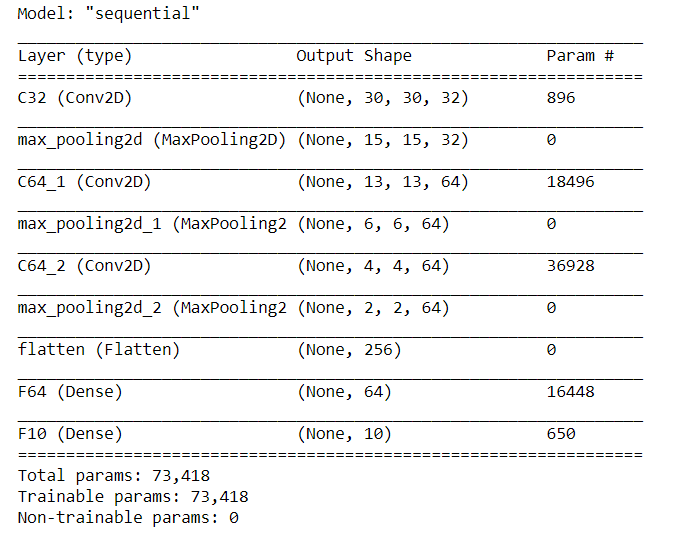
\includegraphics[width=.9\linewidth]{4_1.PNG}
  \caption{Custom function for homography computation}
  \label{fig:sub2}
\end{subfigure}
\begin{subfigure}{0.4\textwidth}
  \centering
  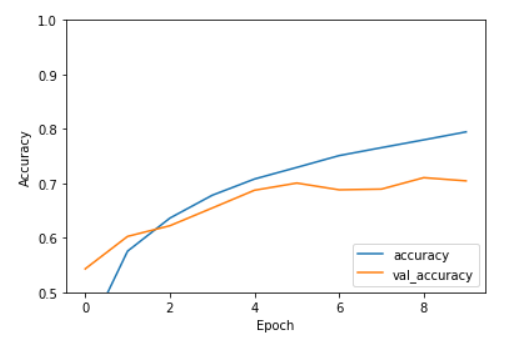
\includegraphics[width=.9\linewidth]{4_2.PNG}
  \caption{Custom function implementation on the images}
  \label{fig:sub2}
\end{subfigure}
\caption{Python implementation of a custom function for homography computation}
\label{fig:test}
\end{figure}

\begin{figure}[H]
\centering
\begin{subfigure}{0.4\textwidth}
  \centering
  \includegraphics[width=.5\linewidth]{4_3.PNG}
  \caption{Input Image - img1.ppm}
  \label{fig:sub2}
\end{subfigure}
\begin{subfigure}{0.4\textwidth}
  \centering
  \includegraphics[width=.5\linewidth]{4_4.PNG}
  \caption{Image 5 - img5.ppm}
  \label{fig:sub2}
\end{subfigure}
\begin{subfigure}{0.4\textwidth}
  \centering
  \includegraphics[width=.8\linewidth]{4_5.PNG}
  \caption{Image 1 warped image}
  \label{fig:sub2}
\end{subfigure}
\caption{Before and after stitching using a custom function}
\label{fig:test}
\end{figure}

Although the above estimations are valid when computing the homoraphy, the resultant warped image suggests that there are significant discontinuities due to various reasons which may include those assumptions. Howsoever, the resultant image is at an acceptable level in which a satisfactory warping is stitched. The black outlines are due to the destination image dimensions specified in the inbuilt \textit{warpPerspective} function. 

\paragraph*{Problem 5}
Stitch images using \href{https://github.com/magicleap/SuperGluePretrainedNetwork}{SuperGlue} features instead of mouse-clicked points. Compute the homography though RANSAC or MSAC. Stitch more than two images using mouse-clicked points. Handle the seams. See the original paper \href{http://matthewalunbrown.com/papers/iccv2003.pdf}{here}.

The RANSAC algorithm could be implemented using OpenCV inbuilt \textit{findHomography} using the input argument of \textit{cv2.RANSAC} and \textit{ransacReprojThreshold}. 

\begin{figure}[h!]
    \centering
    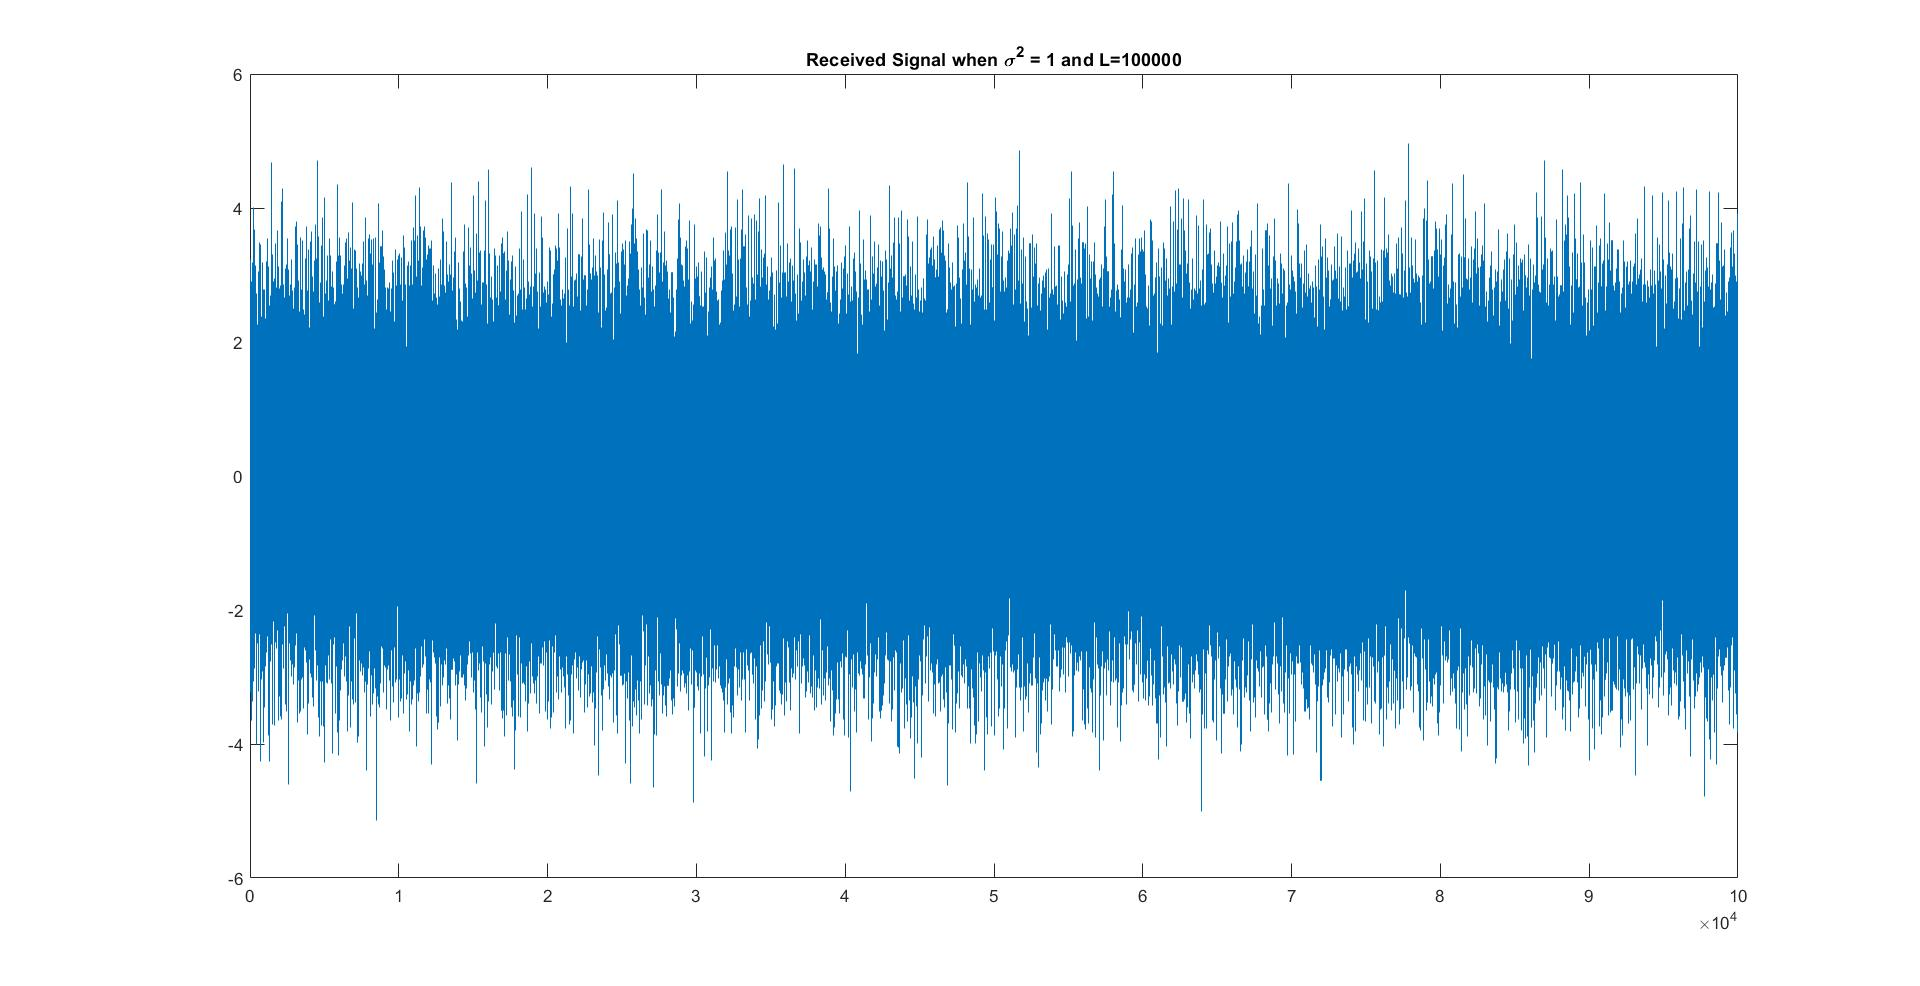
\includegraphics[width=0.90\textwidth]{5_1.PNG}
    \caption{RANSAC algorithmic implementation of homography}
    \label{fig: PaleBlueDot}    
\end{figure}

\begin{figure}[h!]
    \centering
    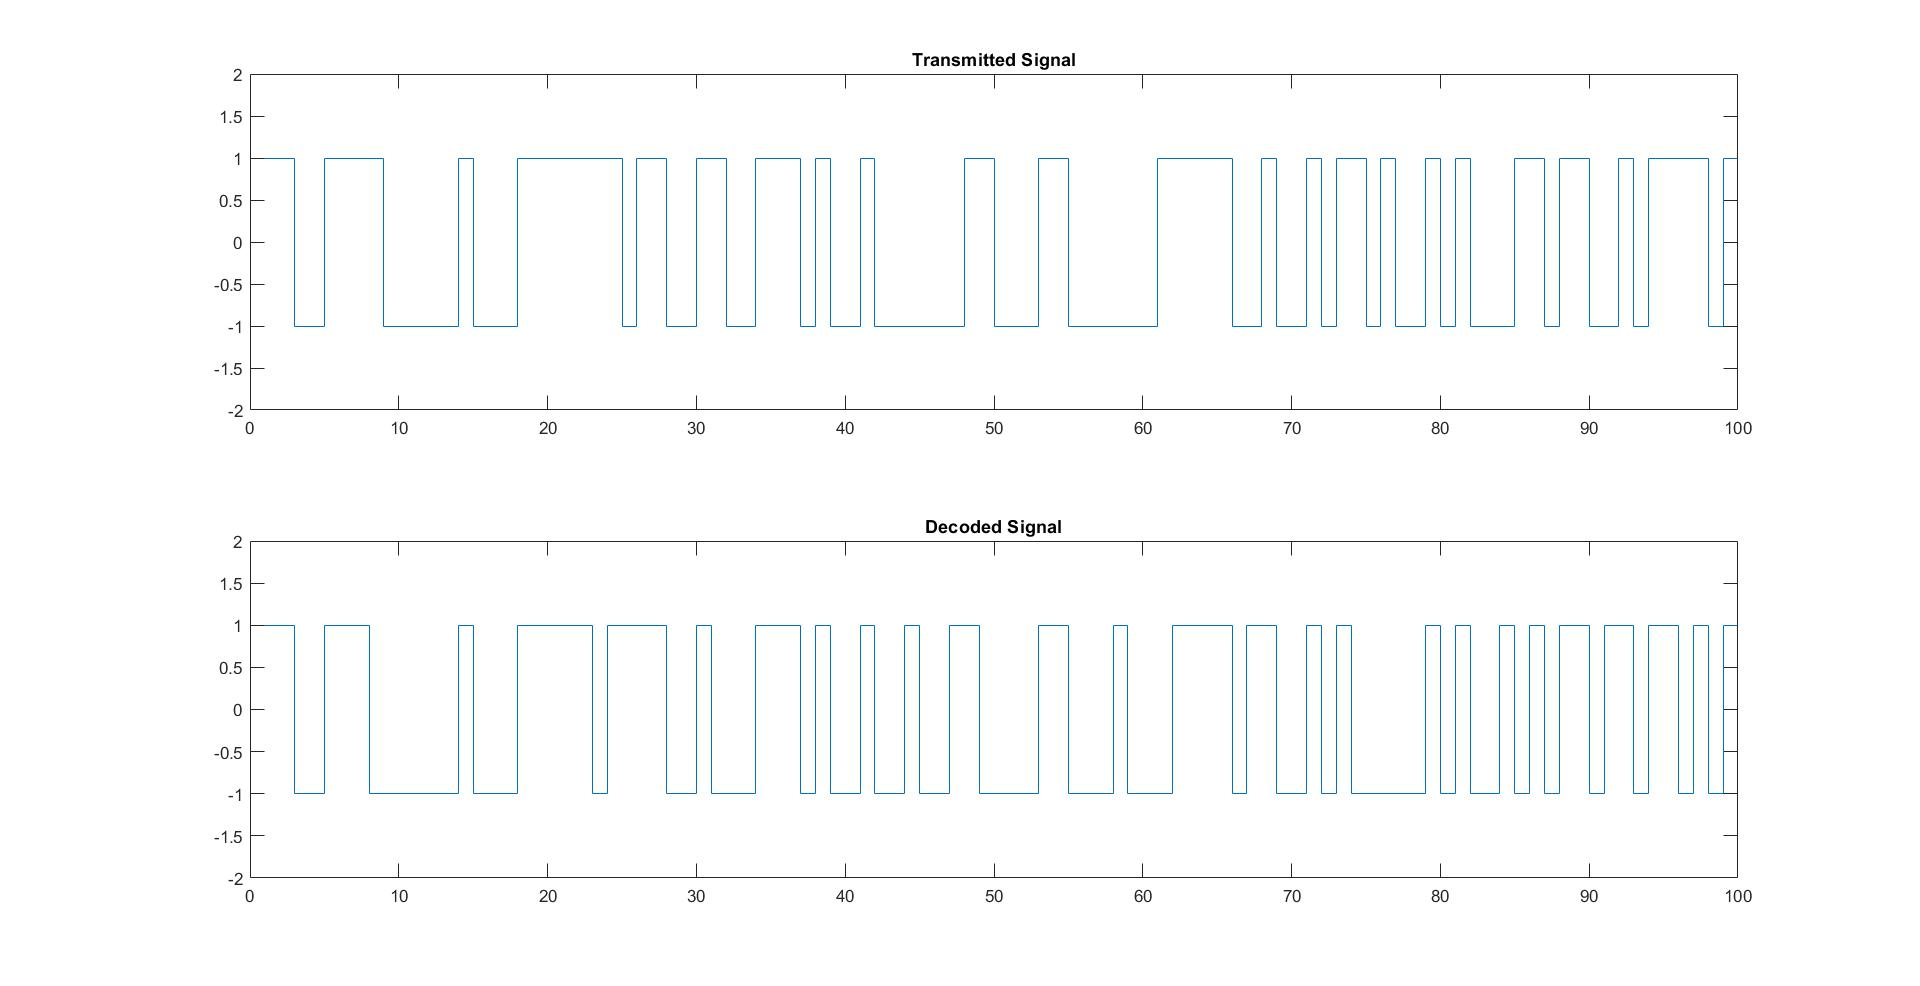
\includegraphics[width=0.50\textwidth]{5_2.PNG}
    \caption{Result image after warped using RANSAC for the stitching in Problem (3)}
    \label{fig: PaleBlueDot}    
\end{figure}



\end{document}

